\chapter{Testing \& Results}
\label{ch:testing_results}
\acresetall


\section{Initialization Phase}

\subsection{Hypothesis}

\subsection{Setup}

\subsection{Procedure}



\section{Route Convergence}

\subsection{Hypothesis}

\subsection{Setup}

\subsection{Procedure}



\section{Results}

\subsection{Initialization Phase}

\begin{figure}[h]
	\centering
	\subfloat[Original B.A.T.M.A.N.]{\label{fig:test_1_original}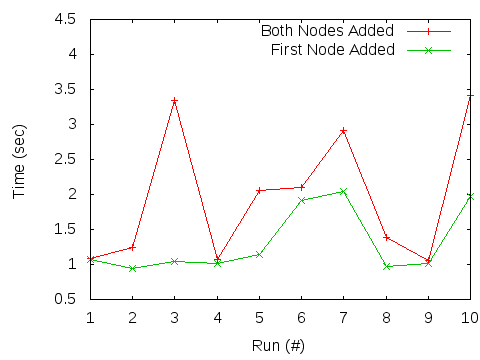
\includegraphics[width=0.5\textwidth]{images/test_1_original.png}}
	\subfloat[Modified B.A.T.M.A.N.]{\label{fig:test_1_secure}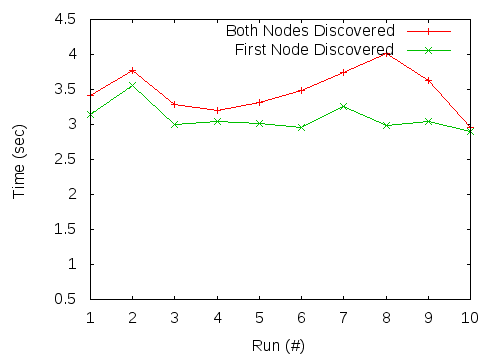
\includegraphics[width=0.5\textwidth]{images/test_1_secure.png}} 
	\caption{In a network of three nodes, the time spent by the \ac{SP} from its first neighbor discovery and until both neighbors are added to its routing table.}
	\label{fig:results_test_1}
\end{figure}

\subsection{Route Convergence}

\begin{figure}[h]
	\centering
	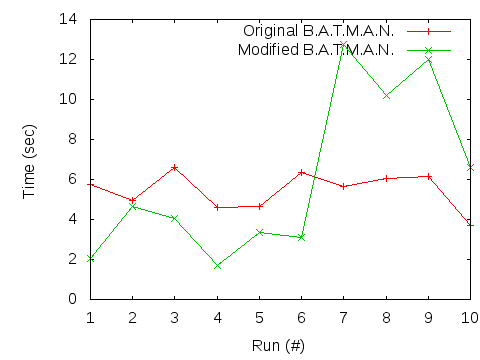
\includegraphics[width=0.8\textwidth]{images/test_2.png}
	\caption{Routing path convergence time observed by a distant source node to another sink node in the network. The source node is only sporadically connected to the network through a mobile intermediate node.}
	\label{fig:results_test_2}
\end{figure}